% !TEX root = ../my_thesis.tex
\newpage
\section{Training des Convolutional Neural Networks}
cnns werden erst modelliert und anschließend traniert.
posenet caffe implementierung
Trainingsdaten sind die synthetischen Daten und Testdaten sind die realen Daten

\subsection{Erhebung der realen Daten}
In der Literatur wurden die realen Daten einer Zone grundsätzlich entlang einer Strecke aufgenommen. Daher wurden für die Aufgabenstellung interessante Aufnahmestrecken in den Gebäudesimulationen festgelegt und anschließend die Aufnahmen so durchgeführt, dass diverse Projekte damit Forschung betreiben können. 

In der Literatur wurden SfM-Methoden eingesetzt, um die Ground-Truth-Daten der realen Aufnahmen zu bestimmen. 
In der vorliegenden Arbeit wurde für die Bestimmung der Ground-Truth-Daten sowie die Aufnahme der Bilder zeitgleich zwei unterschiedliche Kameras der Intel Realsense Reihe verwendet. Eine Intel Realsense T265\footnote{\url{https://www.intelrealsense.com/tracking-camera-t265/} (abgerufen am: 18.07.2019)}, die die Odometrie (Ground-Truth-Daten) mit einer Abweichung von 1\%  über die SfM von zwei Fischaugenkameras und Inertial Measurement Units (\textit{IMU}) ermittelt, wurde eingesetzt. Zudem wurde eine Intel Realsense D435\footnote{ \url{https://www.intelrealsense.com/depth-camera-d435/} (abgerufen am: 18.07.2019)}, die eine 3D Punktwolke, ein Tiefenbild sowie ein RGB-Bild einer Szene liefert, benutzt. Die T265 wurde über die D435 Kamera montiert (siehe Abbildung \ref{fig:t265_d435}). 

Über das Robot Operating System\footnote{\url{https://www.ros.org/about-ros/} (abgerufen am: 18.07.2019)} (\textit{ROS}) Framework wurden die Kameras zeitgleich angesprochen und der Datenfluss der Kameras synchronisiert. Somit beinhaltet jeder Datensatz ein Bild je Fischaugenkamera, ein Tiefenbild, ein RGB-Bild, eine 3D Punktwolke und die dazugehörige Odometrie pro Frame (siehe Abbildung \ref{fig:dataset}). Für die vorliegende Arbeit sind nur die Odometrie-Daten der T265 sowie die RGB-Bilder der D435 relevant.


\begin{figure}[htp]
	\centering
	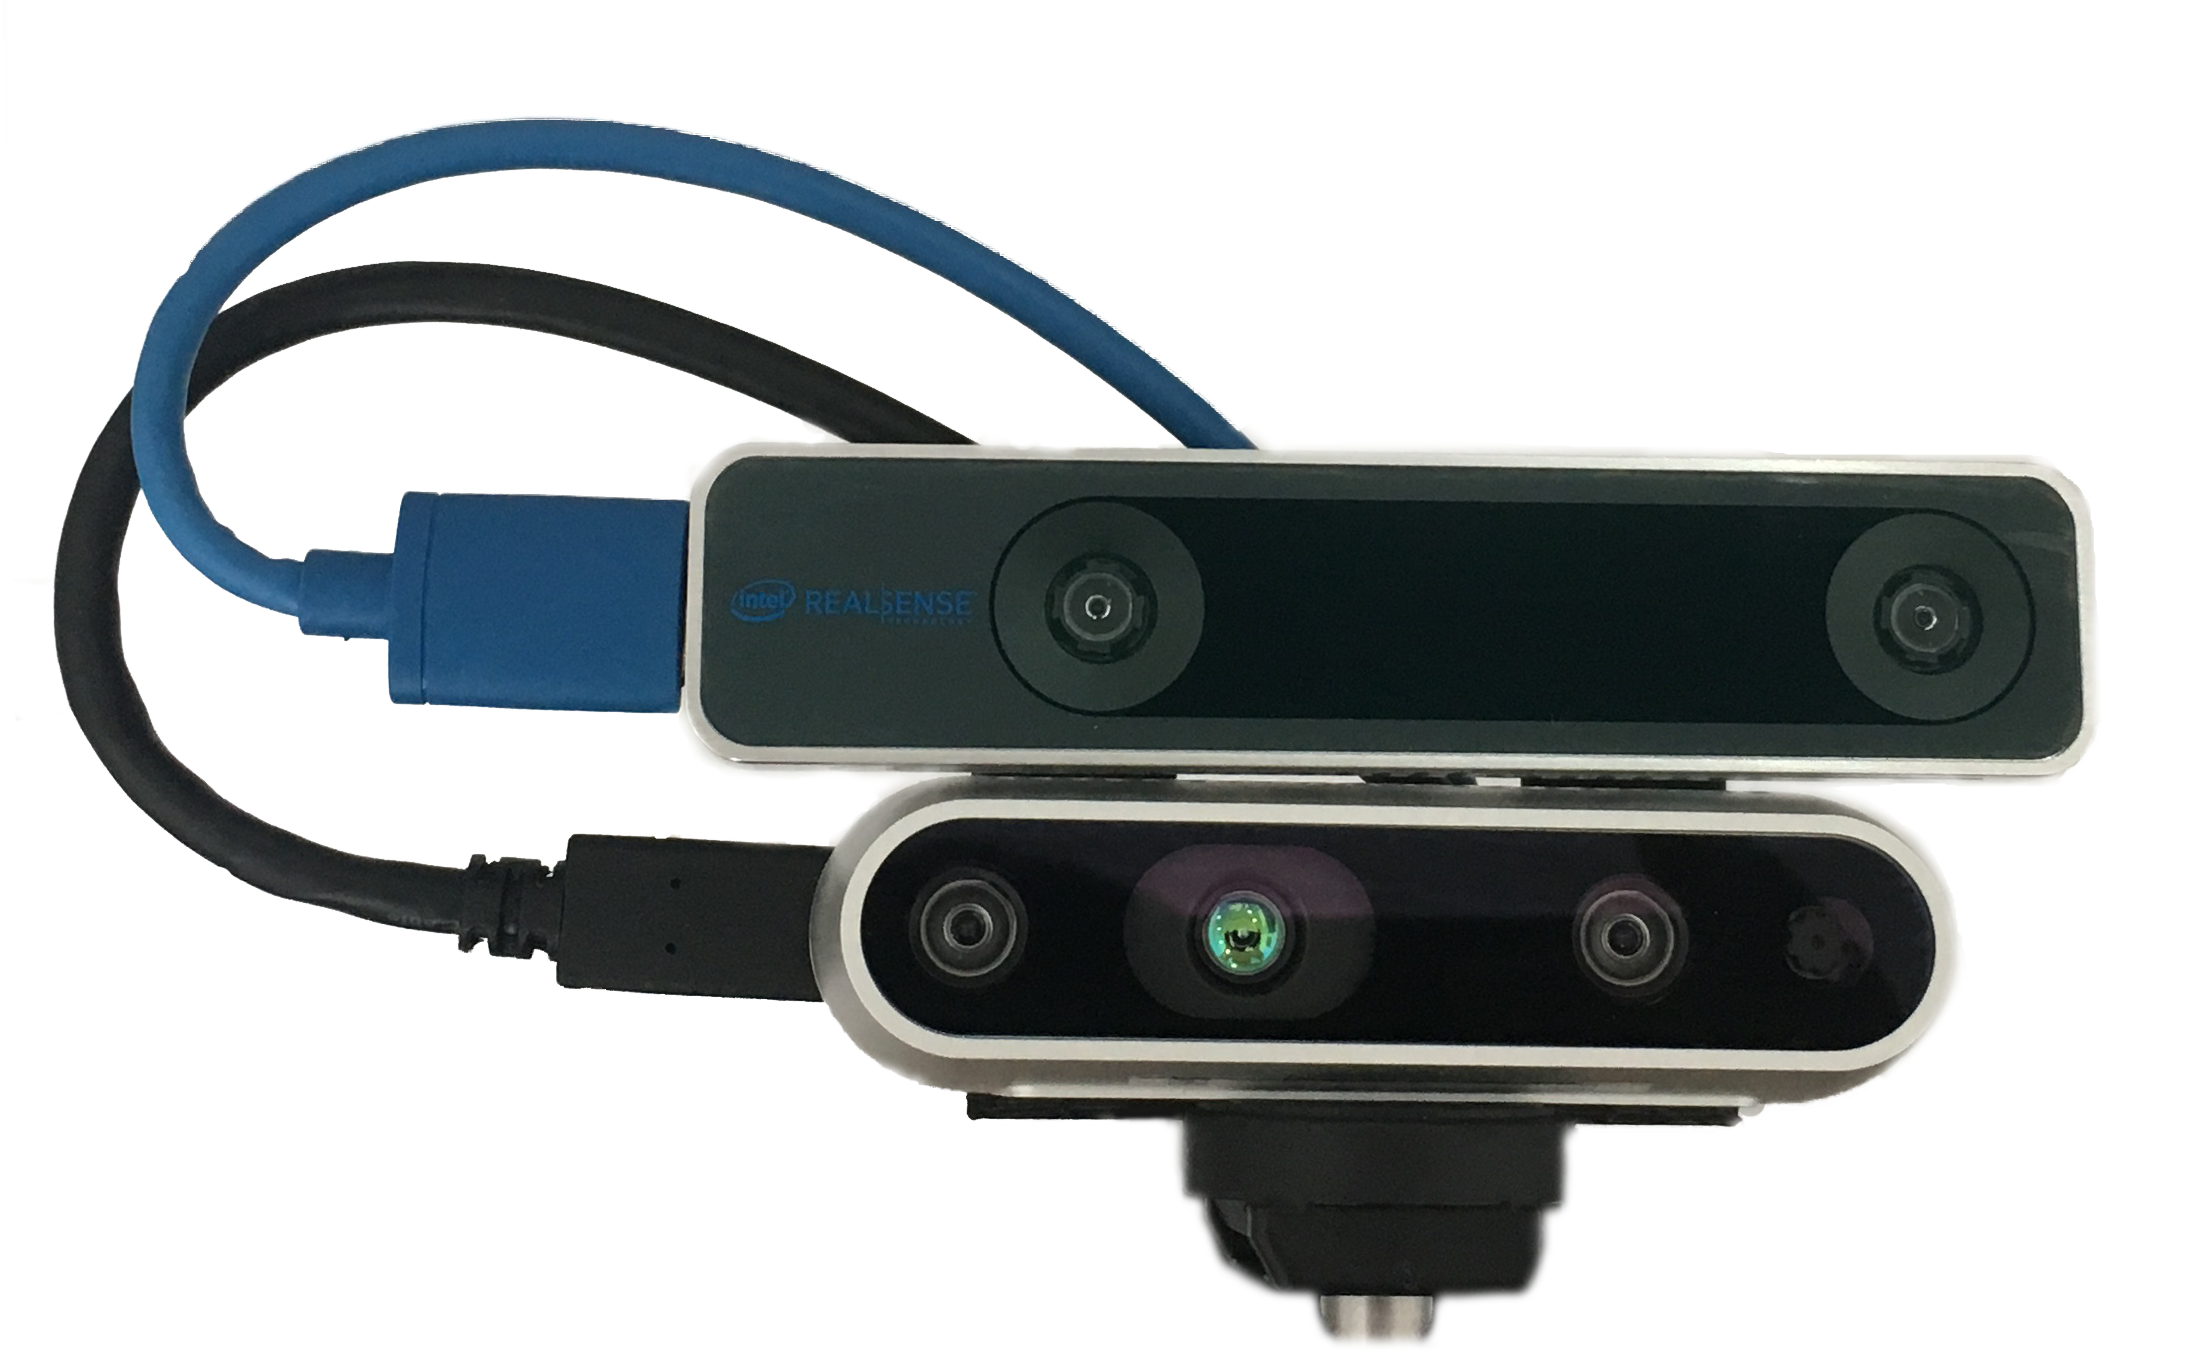
\includegraphics[width=0.5\textwidth]{images/dataset/t265_d435_2.png}
	\caption{Hardware für die Aufnahme der echten Daten. Die Intel Realsense T265 ist oberhalb der Intel Realsense D435 montiert. Das Konstrukt kann auf einer beliebigen universal Stativschraube befestigt werden.  }
	\label{fig:t265_d435}
\end{figure}


\begin{figure}[H]
	\centering
	\begin{subfigure}[b]{0.3\linewidth}
		\centering
		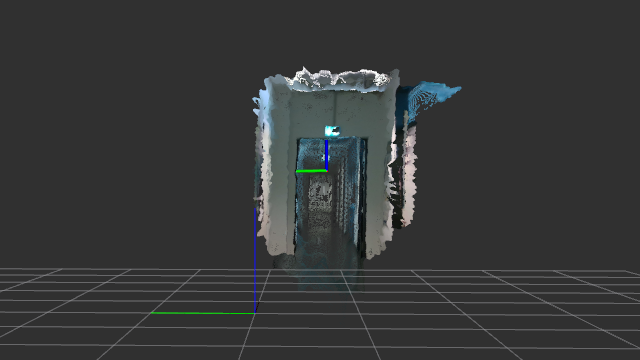
\includegraphics[width=\linewidth]{images/dataset/pointcloud3.png}
		\caption{Odometrie  (T265) + \\ 3D Punktwolke (D435)}
		\label{subfig:odom1}
	\end{subfigure}
	\hfill
	\begin{subfigure}[b]{0.3\linewidth}
		\centering
		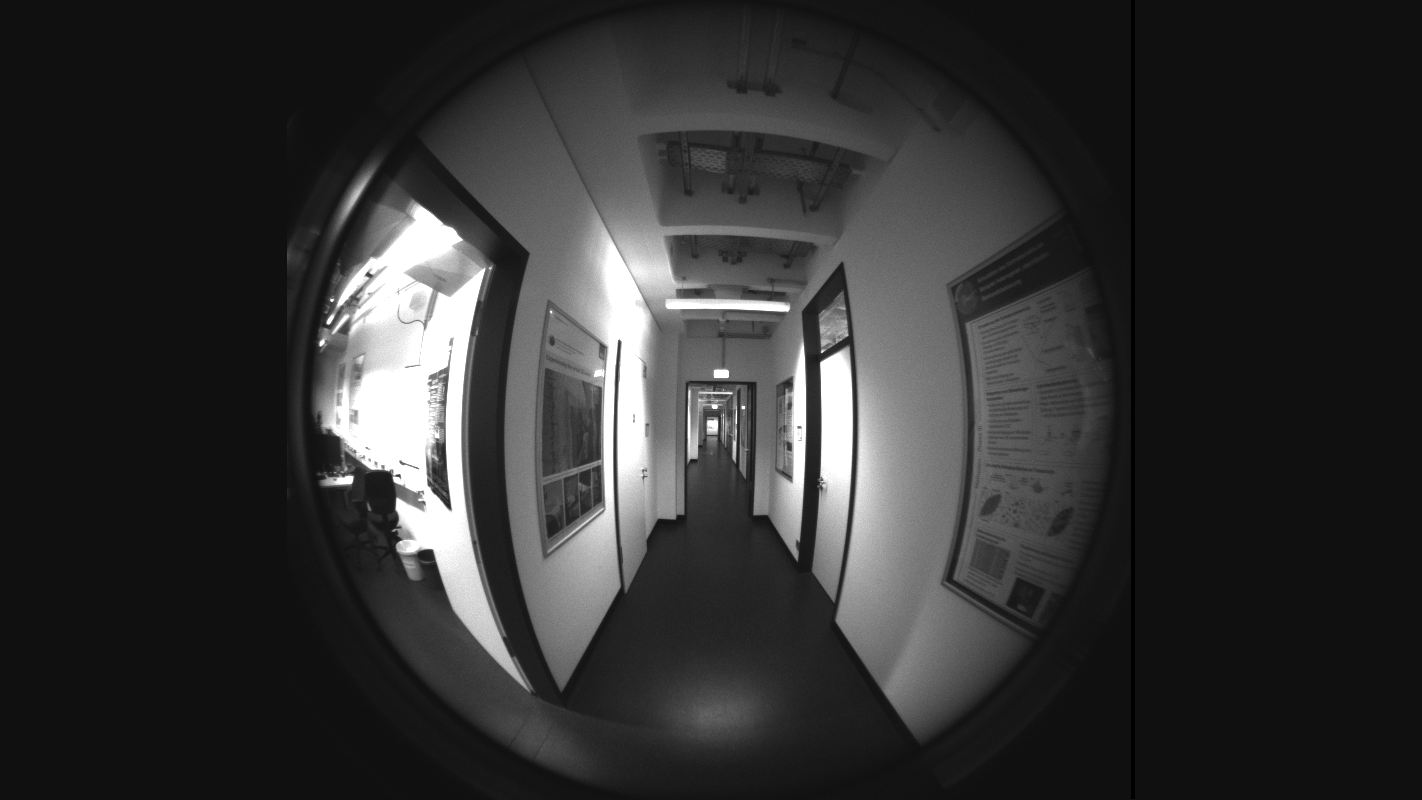
\includegraphics[width=\linewidth]{images/dataset/f1_frame000005.png}
		\caption{Fischaugenkamera 1 \\ (T265)}
		\label{subfig:fisheye1}
	\end{subfigure}
	\hfill
	\begin{subfigure}[b]{0.3\linewidth}
		\centering
		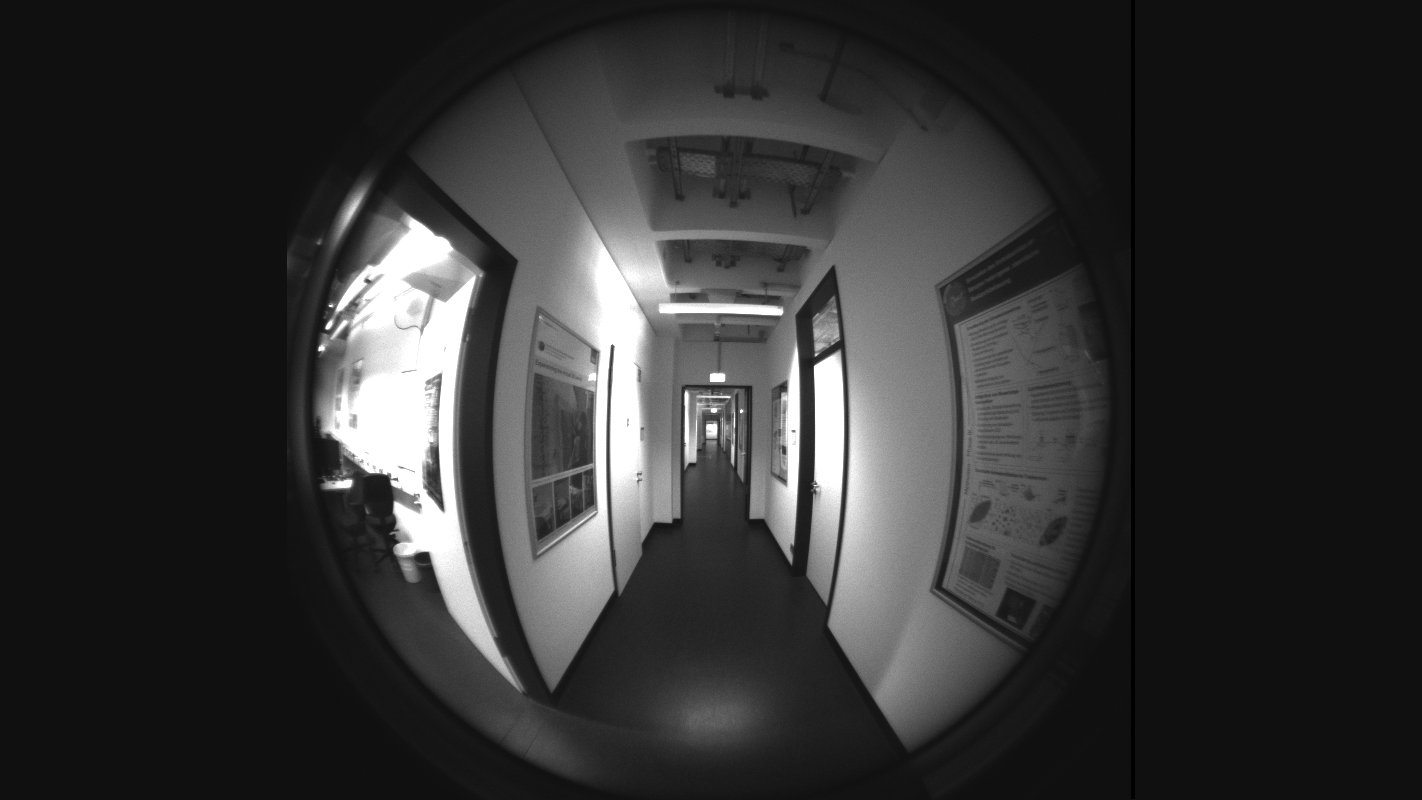
\includegraphics[width=\linewidth]{images/dataset/f2_frame000005.png}
		\caption{Fischaugenkamera 2 \\ (T265)}
		\label{subfig:fisheye2}
	\end{subfigure}
	\medskip
	\begin{subfigure}[b]{0.3\linewidth}
		\centering
		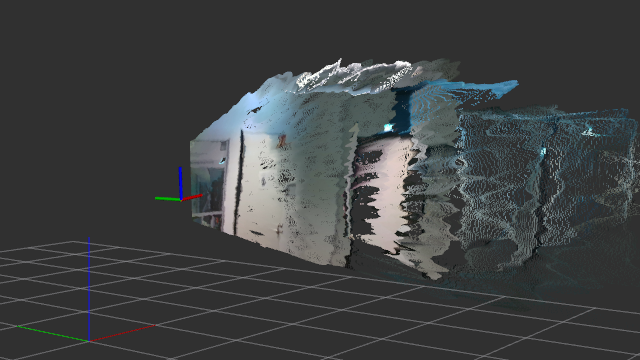
\includegraphics[width=\linewidth]{images/dataset/pointcloud1.png}
		\caption{Odometrie  (T265) + \\ 3D Punktwolke (D435)}
		\label{subfig:odom2}
	\end{subfigure}
	\hfill
	\begin{subfigure}[b]{0.3\linewidth}
		\centering
		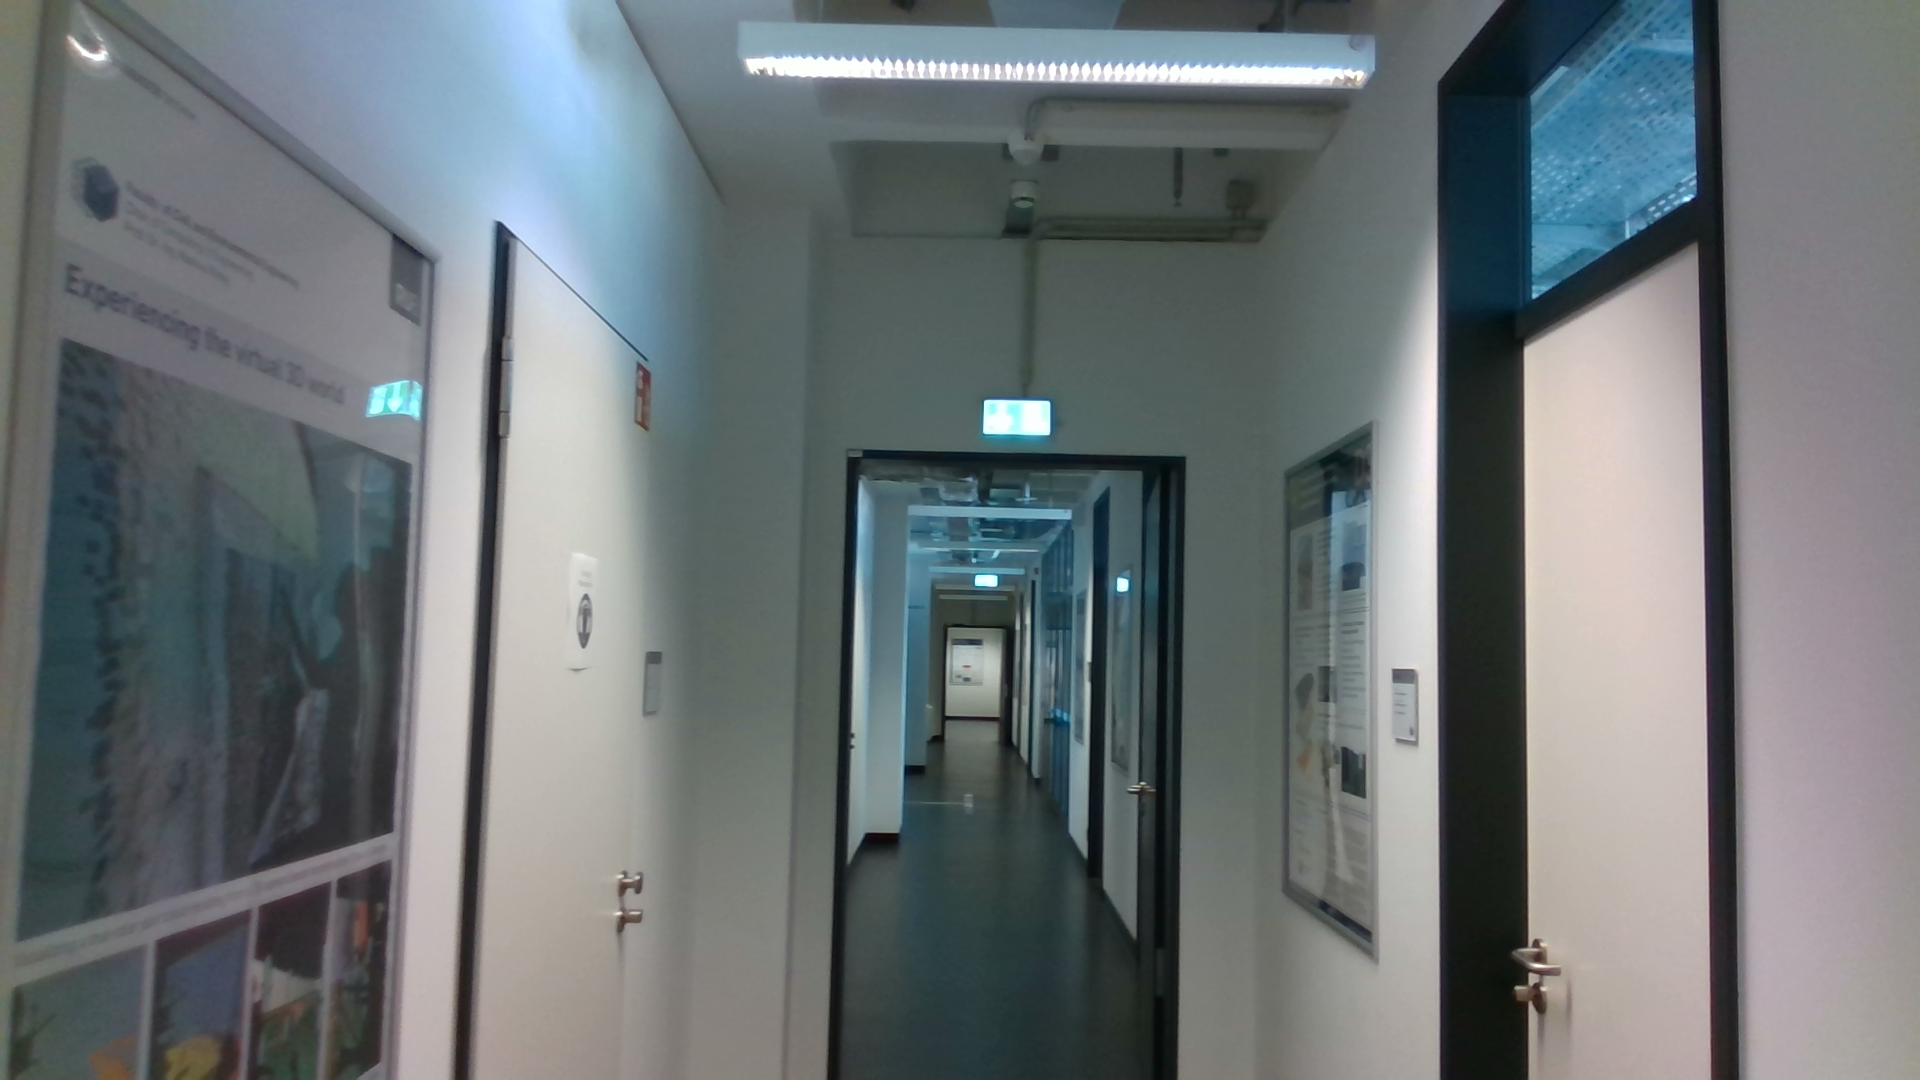
\includegraphics[width=\linewidth]{images/dataset/dc_frame000005.png}
		\caption{RGB-Bild \\ (D435) \hspace*{2cm}}
		\label{subfig:rgb-image}
	\end{subfigure}
	\hfill
	\begin{subfigure}[b]{0.3\linewidth}
		\centering
		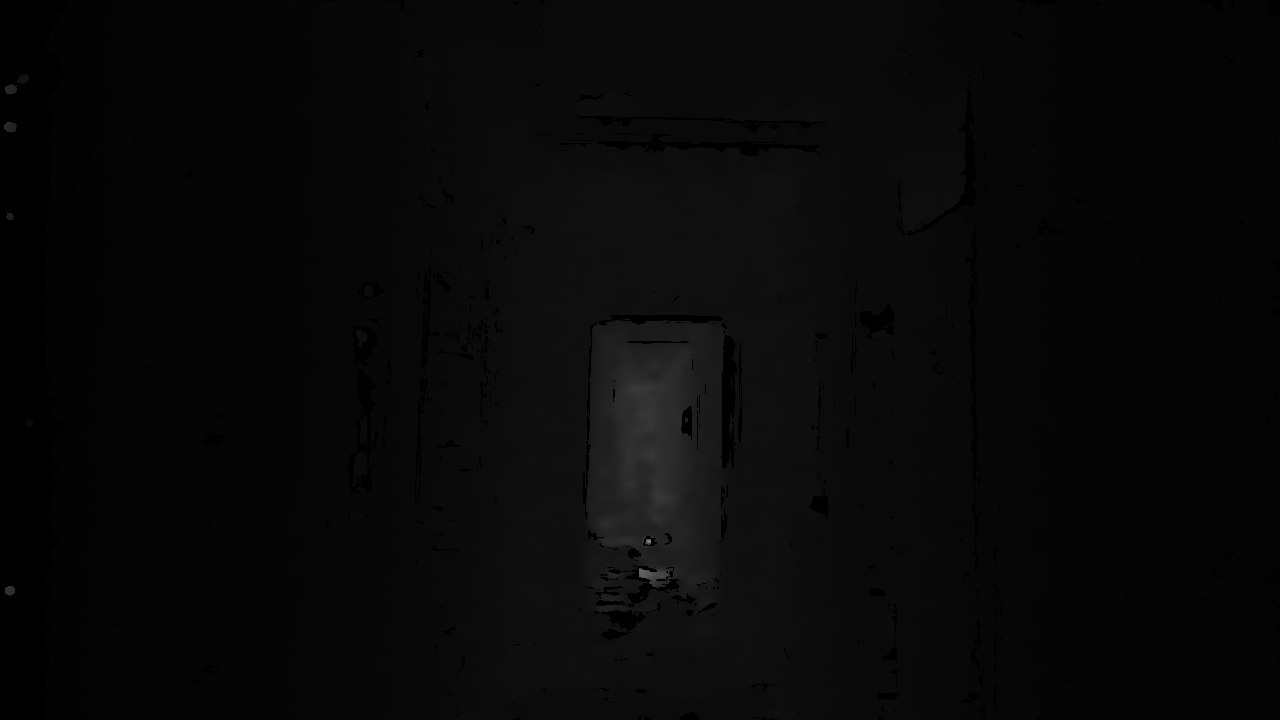
\includegraphics[width=\linewidth]{images/dataset/dt_frame000005.png}
		\caption{Tiefenbild \\ (D435) \hspace*{2cm}}
		\label{subfig:depth-image}
	\end{subfigure}
	\caption{Datensatz pro Frame. \ref{subfig:odom1}  und \ref{subfig:odom2} visualisieren in unterschiedlichen Prespektiven die von der T265 ermittelte Odometrie und die von der D435 erhaltenen 3D Punktwolke. \ref{subfig:fisheye1} und \ref{subfig:fisheye2} sind die von der T265 aufgenommenen Fischaugenbilder. \ref{subfig:rgb-image} ist das RGB-Bil der D435 und \ref{subfig:depth-image} das dazugehörige Tiefenbild. }
	\label{fig:dataset}
\end{figure}


\subsection{Generierung der synthetischen Daten}
\label{subsec:generate_synth_images}

Die Gebäuden wurden in Blender\footnote{\url{https://www.blender.org} (aufgerufen am: 20.07.2019)} Version 2.79b simuliert. Die Strecke der echten Aufnahmen wurden in den Simulationen schwankungslos auf einer konstanten Höhe von 1.70$m$ imitiert.


Die intrinsischen Daten der D435 RGB-Kamera wurden auf die virtuellen Kameras übertragen. Es wurde entlang der Strecke in 0.05$m$ Intervallen und mit einer $\pm$10° Neigung in je Y- und Z-Achse Bilder (siehe Abbildung ...) mit korrespondierenden Ground-Truth-Daten aufgenommen.

Insgesamt wurden drei synthetische Datensätze je Strecke erzeugt, die sich in ihrer Beschaffenheit von \begin{enumerate*}[label=\alph*)]
	\item karikaturistisch zu
	\item karikaturistische Kantenbilder hin über zu
	\item fotorealistisch
\end{enumerate*} unterscheiden. Bei der Generierung der a) karikaturistischen und c) fotorealistischen Datensätzen wurde die Beleuchtung aus einem Netz von Punktlichtquellen nachgestellt. Die a) karikaturistische und c) fotorealistische Datensätze unterscheiden sich ausschließlich in den Render-Engines.
Für die Erzeugung der b) karikaturistischen Kantenbilder wurde eine konstante Beleuchtung verschaffen und die Kanten über Blender markant sichtbar konfiguriert. Der a) karikaturistische Datensatz sowie die b) Kantenbilder wurde über die Render-Engine \textit{Blender Render} und der c) fotorealistischer Datensatz über die \textit{Cycles-Engine} generiert.


% TODO: bild von den neigungen.

\subsection{Verarbeitung der Daten}
// gradienten\\

Synthetische Bilder, wie sie in  \ref{subsec:generate_synth_images} generiert werden, haben keine realitätsnahe Erscheinung, minimale Texture und 


Bei der Erzeugung von Gradientenbilder gehen einerseits wichtige Informationen im Hinblick auf das Ursprungsbild verloren, andererseits bleiben wichtige Informationen wie z.B. die geometrische Struktur erhalten.


\vspace{\fill}
\begin{figure}[htp]
	\centering
	\begin{subfigure}[b]{0.48\linewidth}
		\centering
		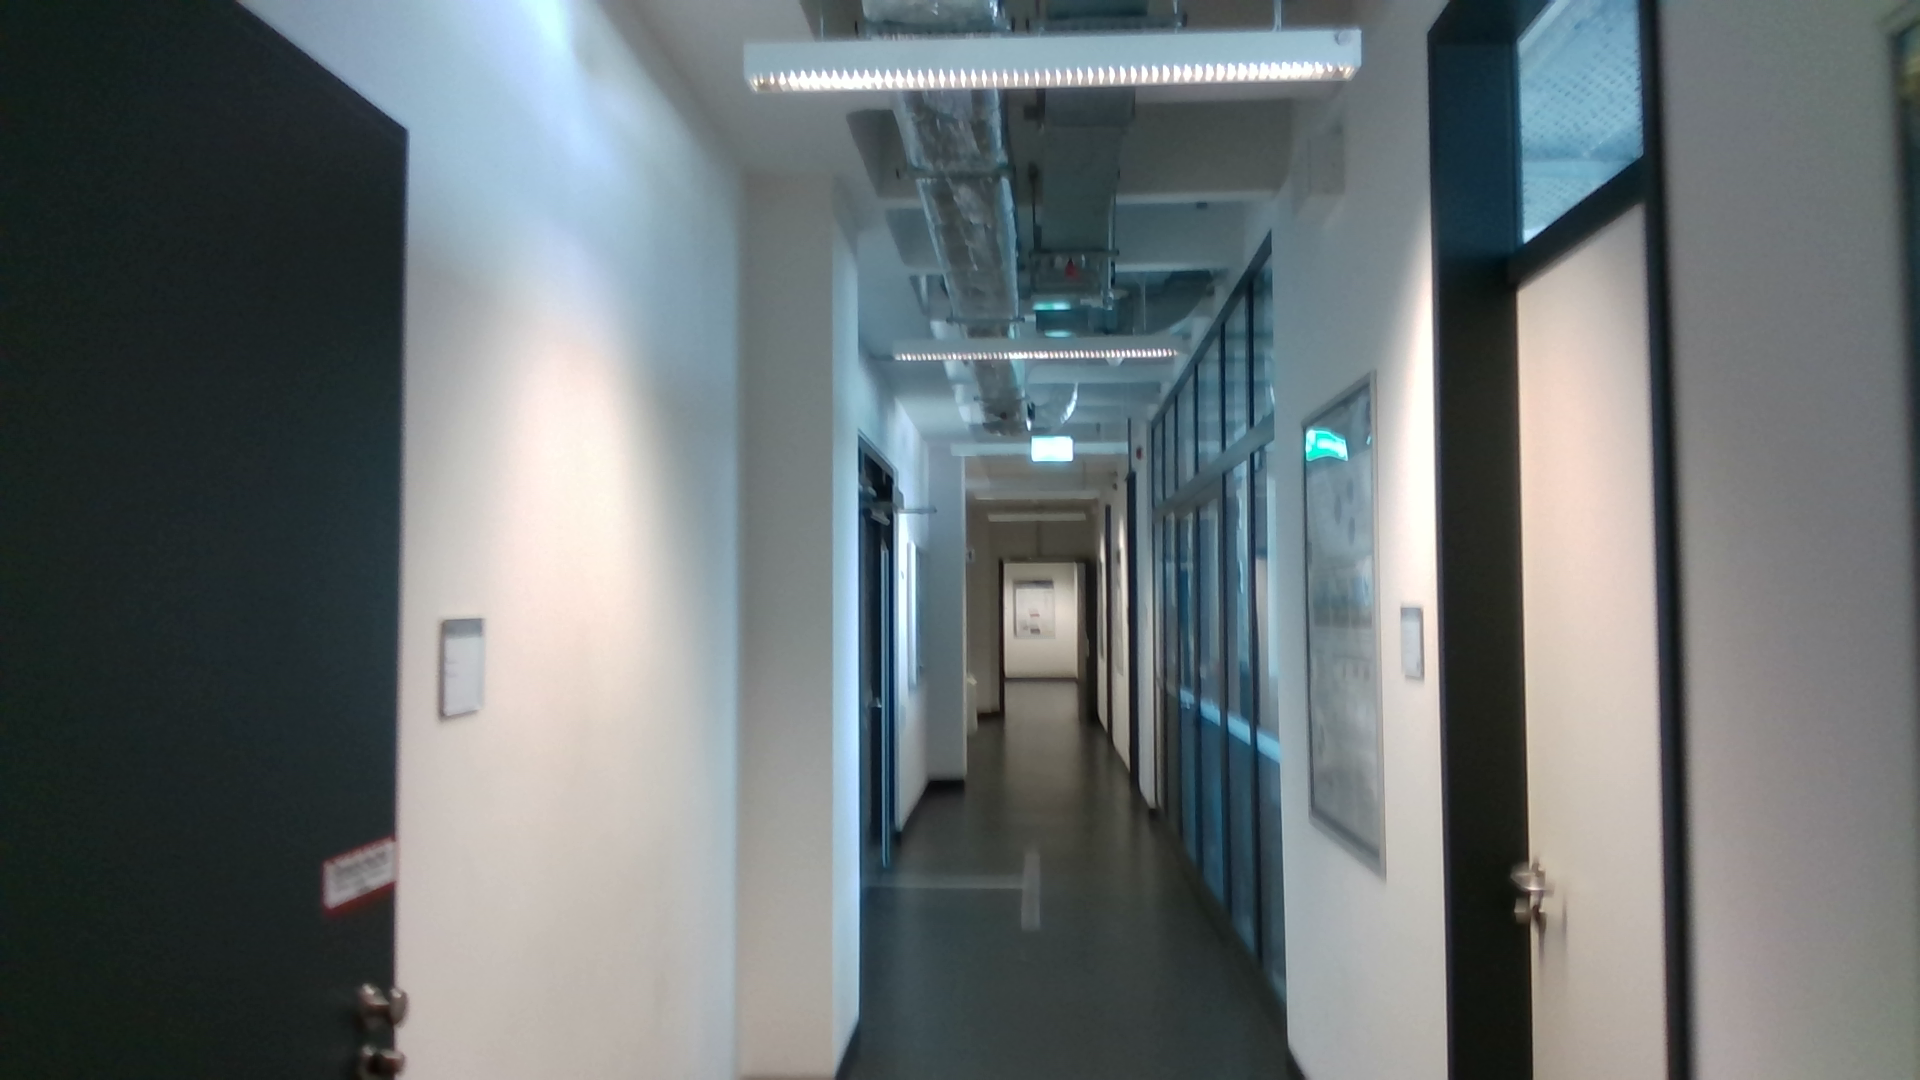
\includegraphics[width=\linewidth]{images/example/r000305.png}
		\caption{reale Aufnahme}
		\label{subfig:real}
	\end{subfigure}
	\hfill
	\begin{subfigure}[b]{0.48\linewidth}
		\centering
		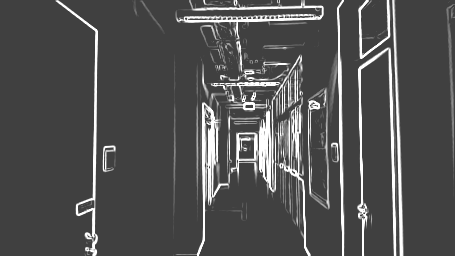
\includegraphics[width=\linewidth]{images/example/rg000305.png}
		\caption{Gradientenbild von \ref{subfig:real}}
	\end{subfigure}
	\hfill
	\begin{subfigure}[b]{0.48\linewidth}
		\centering
		\includegraphics[width=\linewidth]{images/example/b00643.png}
		\caption{karikaturistische Simulation}
		\label{subfig:cartoonish}
	\end{subfigure}
	\hfill
	\begin{subfigure}[b]{0.48\linewidth}
		\centering
		\includegraphics[width=\linewidth]{images/example/bg00643.png}
		\caption{Gradientenbild von \ref{subfig:cartoonish}}
	\end{subfigure}
	\hfill
	\begin{subfigure}[b]{0.48\linewidth}
		\centering
		\includegraphics[width=\linewidth]{images/example/e00643.png}
		\caption{karikaturistisches Kantenbild}
		\label{subfig:edge}
	\end{subfigure}
	\hfill
	\begin{subfigure}[b]{0.48\linewidth}
		\centering
		\includegraphics[width=\linewidth]{images/example/eg00643.png}
		\caption{Gradientenbild von \ref{subfig:edge}}
	\end{subfigure}
	\hfill
	\begin{subfigure}[b]{0.48\linewidth}
		\centering
		\includegraphics[width=\linewidth]{images/example/c00643.png}
		\caption{fotorealistisch Simulation}
		\label{subfig:photorealistic}
	\end{subfigure}
	\hfill
	\begin{subfigure}[b]{0.48\linewidth}
		\centering
		\includegraphics[width=\linewidth]{images/example/cg00643.png}
		\caption{Gradientenbild von \ref{subfig:photorealistic}}
	\end{subfigure}
	\caption{Beispielhafte Bilder für jede Art von Daten und die dazu korrespondierenden Gradientenbilden.}
	\label{fig:dataset_preprocess}
\end{figure}
\vspace{\fill}

\subsection{Trainingsparameter}
optimizer, beta,
learningrate,
weights decay, anz. data; ...